\chapter{Probabilistically}

\section{Probability that SS remains at home}

Finding the probability of SS remaining at home after taking $2n$ steps is the same as finding the probability of heads showing up as many times as tails after $2n$ flips or vice-versa. This is because for SS to remain at the initial point after walking randomly, the distance traveled in each direction must be the same so they cancel out. Since the step size is the same for both directions, the number of steps taken in each direction must also be the same as well.

Since SS is walking $2n$ steps each day, the number of steps he is taking each direction must be $n$. Thus, we can define the probability of him remaining at home after his random walks can simply be found using binomial distribution.

\begin{equation}
\begin{aligned}
	Pr[\#H = n]
		&=\binom{2n}{n}\left(\frac{1}{2}\right)^n\left(\frac{1}{2}\right)^n \\
		&=\binom{2n}{n}\left(\frac{1}{2}\right)^{2n} \equiv \frac{(2n)!}{(n!)^2 \cdot 2^{2n}}
\end{aligned}
\end{equation}

\section{Expected number of times SS arrives home}

While there is a closed form out there for calculating the expected number of times SS returns home in the $2n$ steps,
we will use Monte Carlo simulation to show us the trend \textit{because my brain is too smooth for math right now}.

\subsection*{Simulation Setup}

For $n = 1, 2, \ldots, 1000$, have Python create an array with length $2n$ by randomly picking an element from $\{-1, 1\}$.
Then, compute the cumulative sum array of the original array.
In the cumulative sum array, an occurrence of $0$ is an occurrence of SS passing his home. Thus, we count the number of $0$s in the array and that would be the number times he passes his home in $2n$ steps. Repeat this simulation 10,000 times per each $n$.

\newpage

\subsection*{Results of the simulation}

\begin{figure}[h]
	\centering
	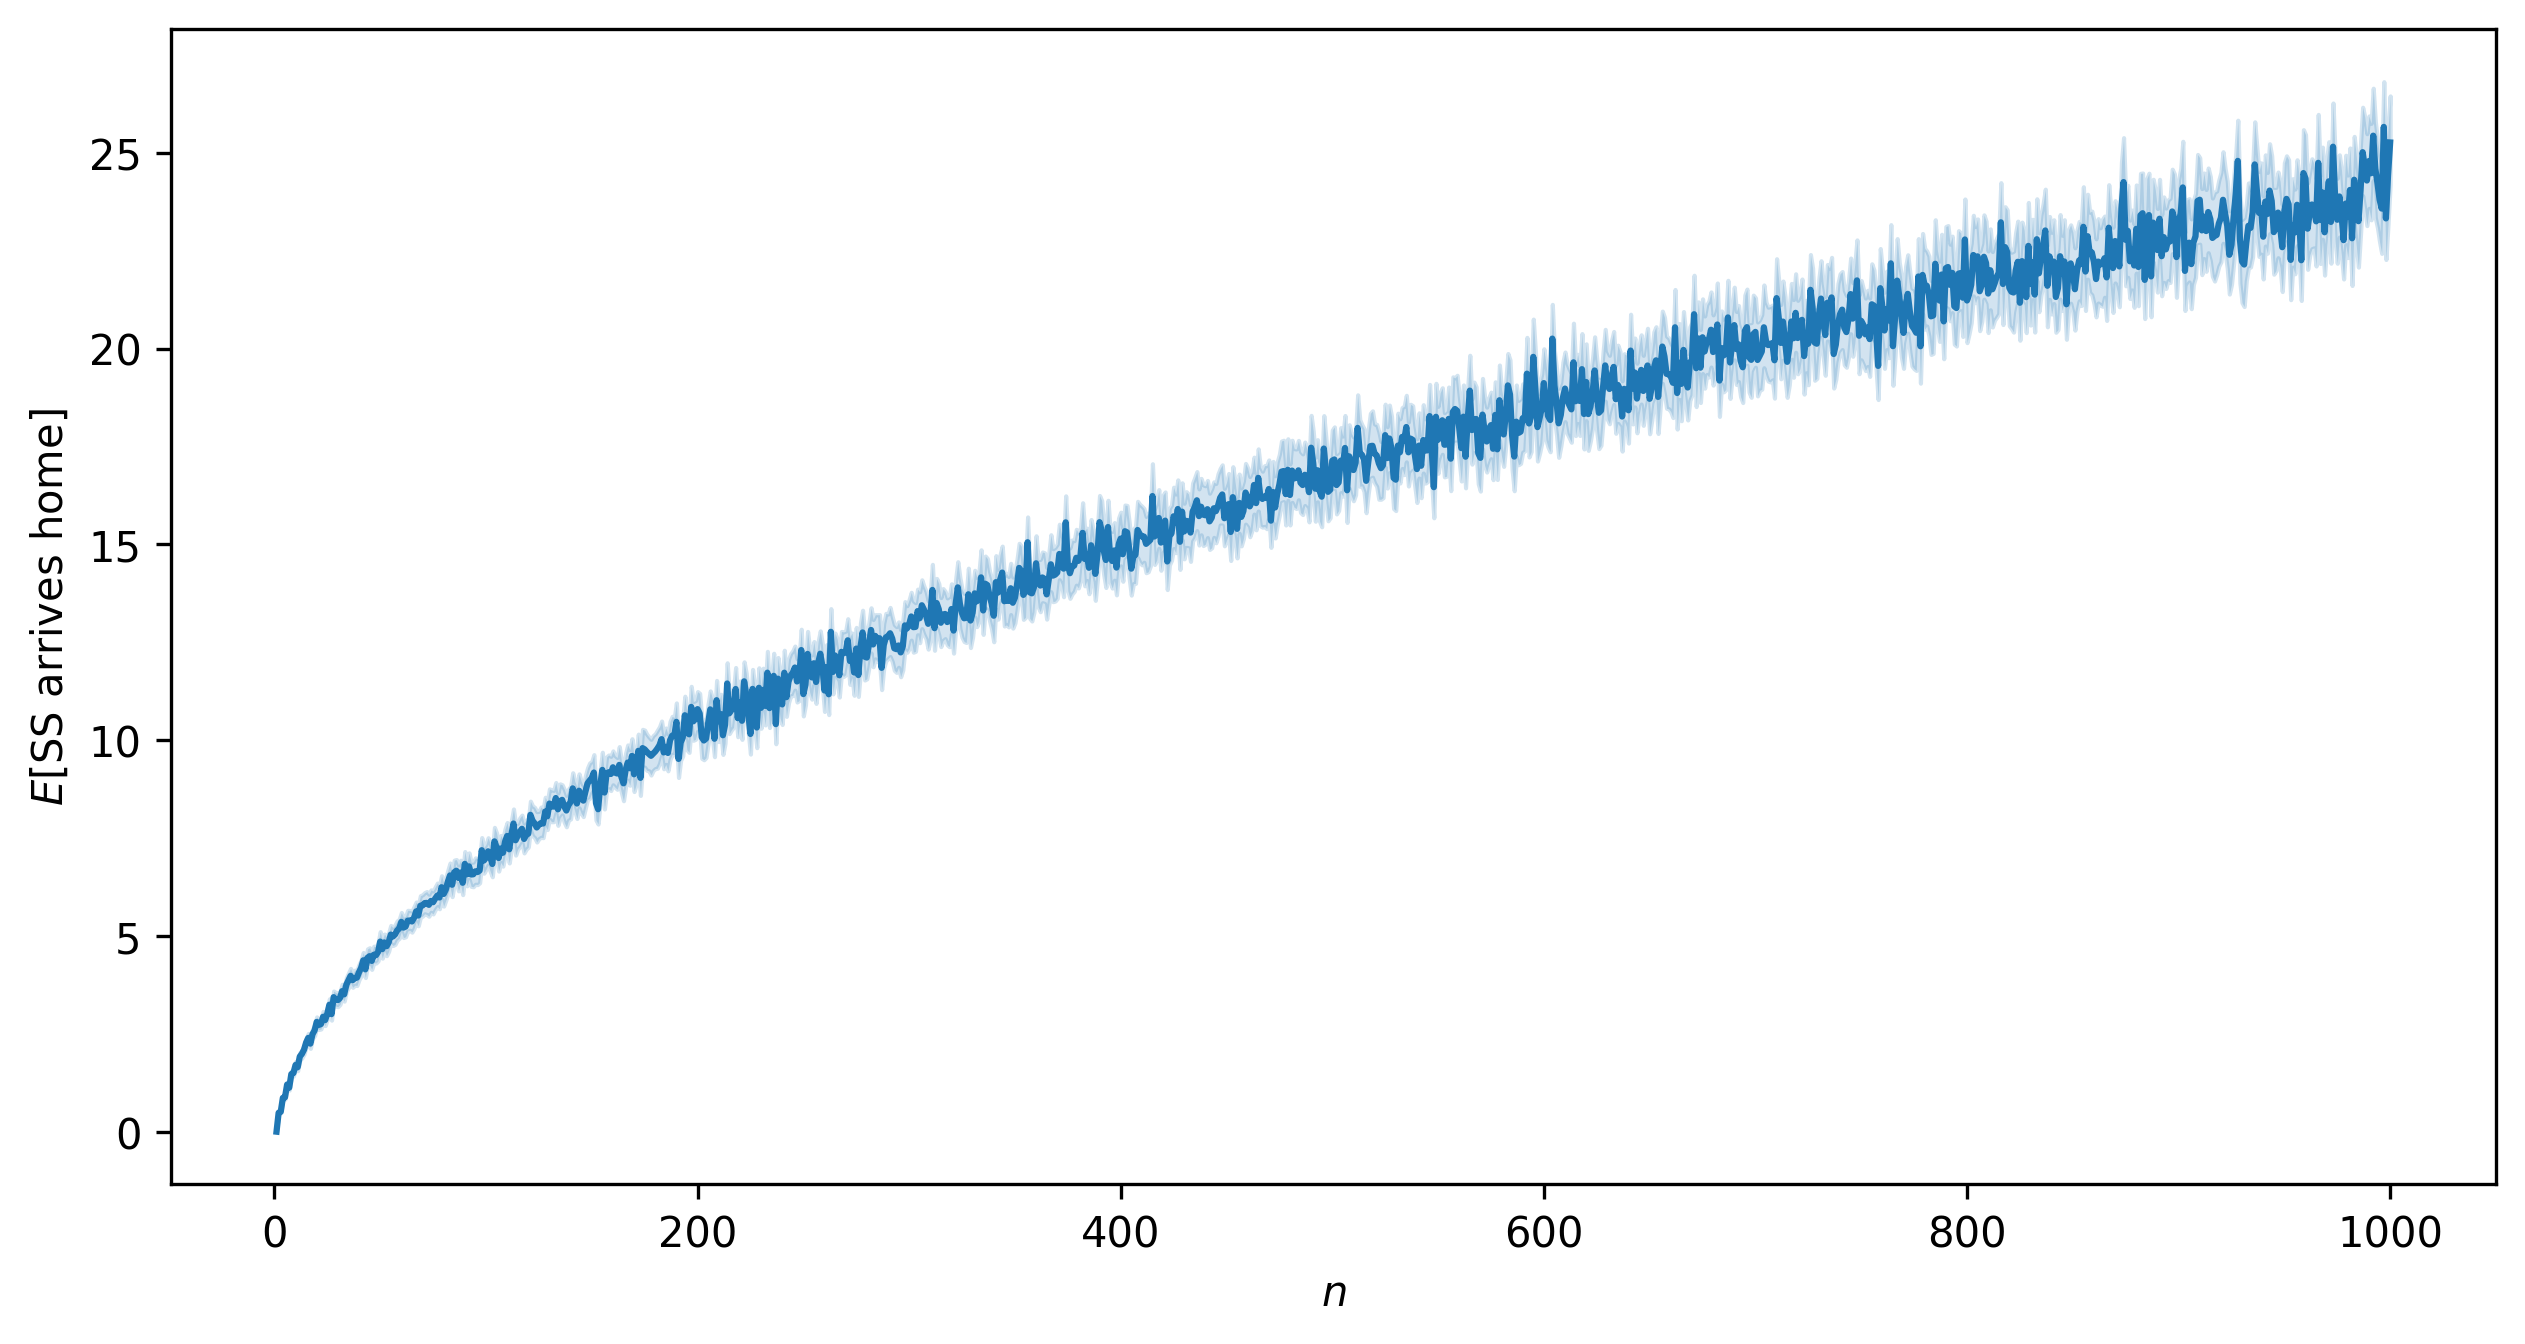
\includegraphics[width=0.8\textwidth]{graphics/02-arriveshome.png}
	\caption{Average number of times SS passes his home}
\end{figure}

An interesting observation we can make is that the average number of time SS passes his home grows logarithmically in relation to $n$.
This gives us some idea on how to fit this line.

\subsection*{Indulging my curiosity}

Finally, because I still want an easy way to compute this (and just extremely curious), I also fitted a line to the results of the simulations.
The function $L(n)$ of the line is the following where $n$ is, well, $n$ from the problem.

\begin{equation}
\begin{aligned}
	&& L(n) &= r \cdot \log(n + h) + c \\
	&\text{where}\ & r &= 13.11223545502508 \\
	&& h &= 231.39007884222403 \\
	&& c &= -69.43227653593898
\end{aligned}
\end{equation}

\begin{figure}[h]
	\centering
	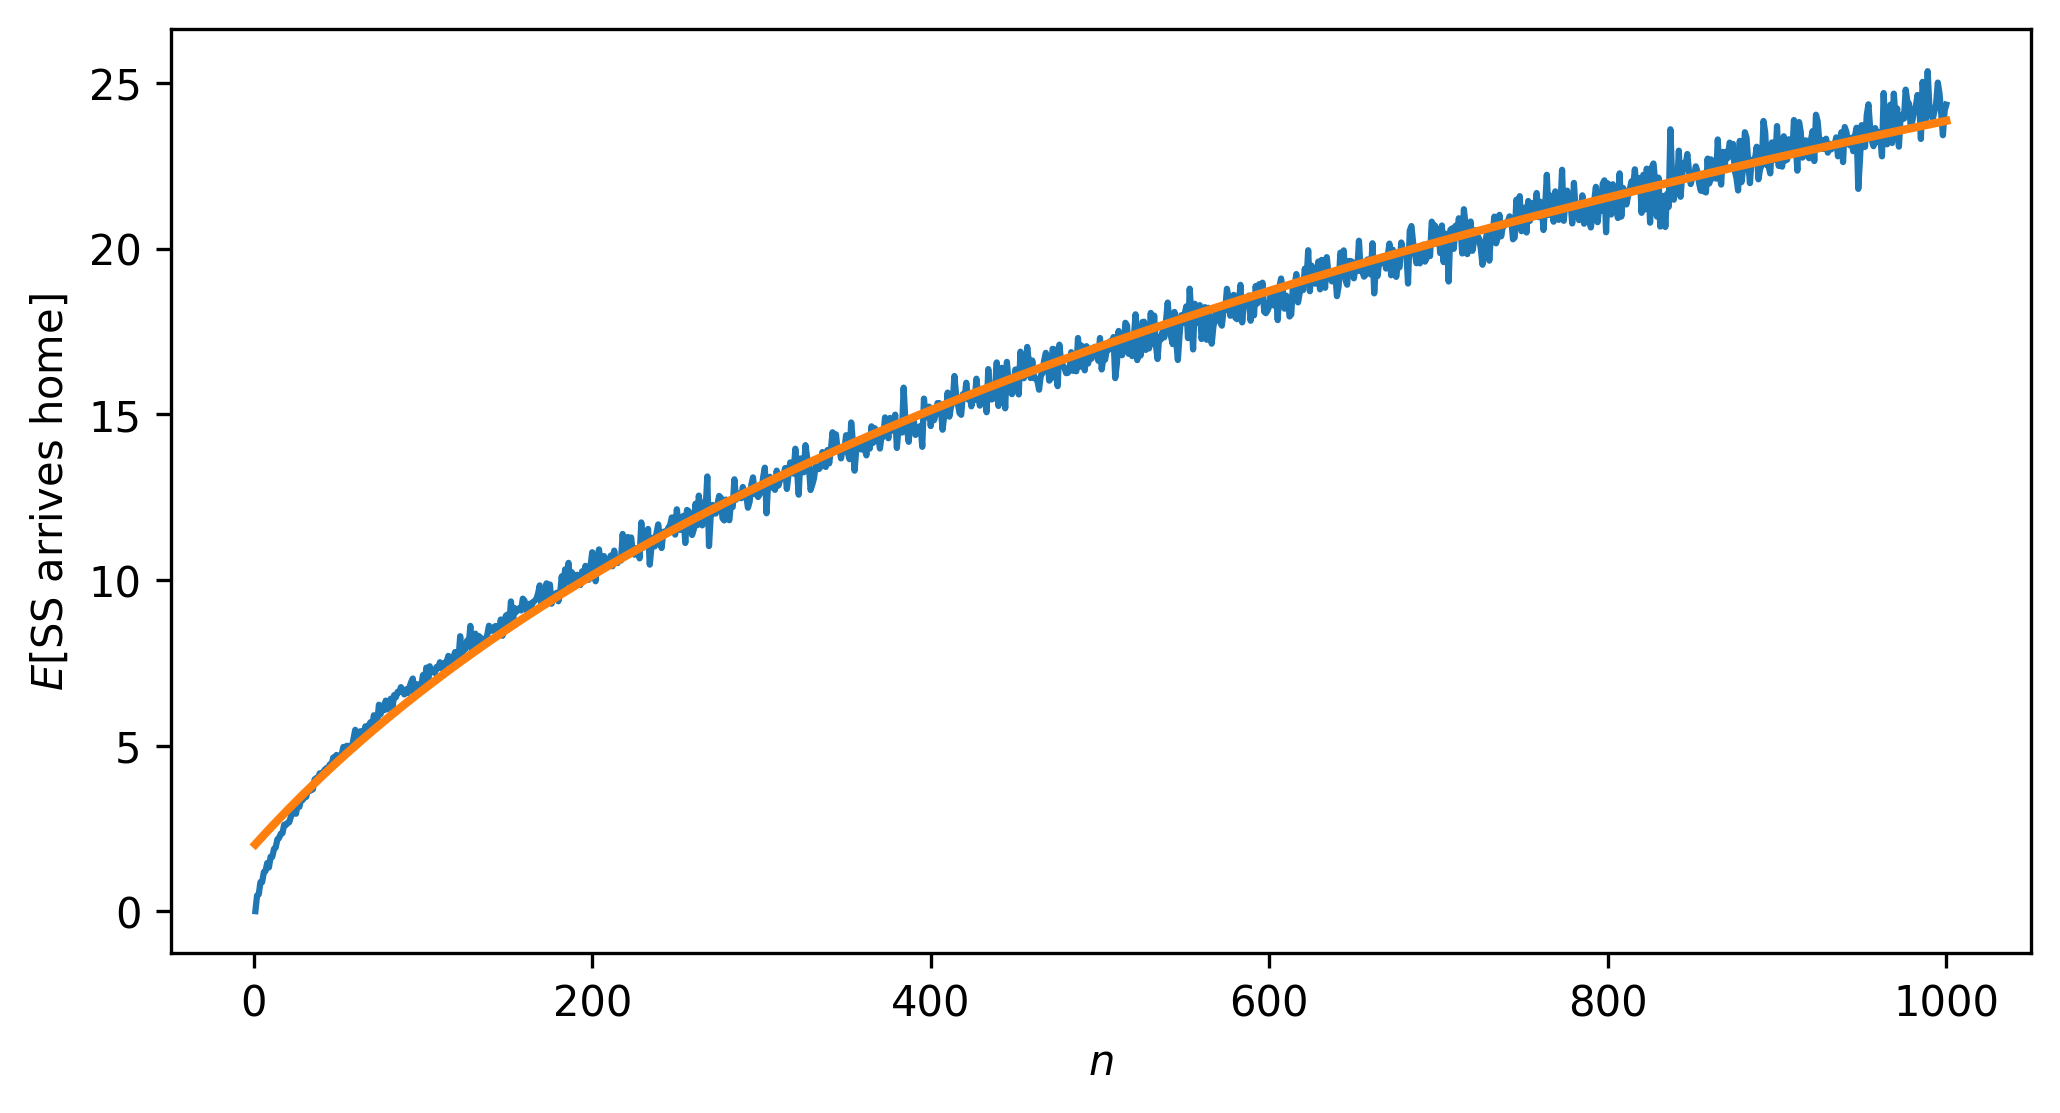
\includegraphics[width=0.8\textwidth]{graphics/02-fittedline.png}
	\caption{Fitted line against the results from the simulations}
\end{figure}

Although it doesn't perfectly fit the line, I think it is good enough for a quick experiment.
